\documentclass{sig-alternate}
%\documentclass[conference]{IEEEtran}
%\documentclass[conference,final]{IEEEtran}

%\usepackage[numbers, sort, compress]{natbib}
\usepackage{graphicx}
\usepackage{amsmath}
\usepackage{amssymb}
\usepackage{color}
\usepackage{ifpdf}
%\usepackage{mdwlist}

%\usepackage{dcolumn}
\usepackage{float}
\usepackage[utf8]{inputenc}
\usepackage{multirow}
\usepackage{rotating}
\usepackage{subfigure}



%\usepackage[numbers, sort, compress]{natbib}
%\usepackage{latex8}
%\usepackage{float}
%\usepackage{times}    
\usepackage{url}
\usepackage{booktabs}
\usepackage{listings}   
\usepackage{paralist}    
\usepackage{wrapfig}    
%\usepackage[footnotesize,it]{caption}
\usepackage{multirow}
\usepackage{ifpdf}
%\usepackage{srcltx}
%\usepackage{subfigure}
\usepackage{xspace}
\usepackage{keyval}  
\usepackage{color}
\usepackage{comment}

\definecolor{listinggray}{gray}{0.95}
\definecolor{darkgray}{gray}{0.7}
\definecolor{commentgreen}{rgb}{0, 0.4, 0}
\definecolor{darkblue}{rgb}{0, 0, 0.4}
\definecolor{middleblue}{rgb}{0, 0, 0.7}
\definecolor{darkred}{rgb}{0.4, 0, 0}
\definecolor{brown}{rgb}{0.5, 0.5, 0}

\usepackage[normalem]{ulem}
\makeatletter
\def\cyanuwave{\bgroup \markoverwith{\lower3.5\p@\hbox{\sixly \textcolor{cyan}{\char58}}}\ULon}
\def\reduwave{\bgroup \markoverwith{\lower3.5\p@\hbox{\sixly \textcolor{red}{\char58}}}\ULon}
\def\blueuwave{\bgroup \markoverwith{\lower3.5\p@\hbox{\sixly \textcolor{blue}{\char58}}}\ULon}
\font\sixly=lasy6 % does not re-load if already loaded, so no memory problem.
\makeatother

\newif\ifdraft
\drafttrue
\ifdraft
\usepackage{xcolor}
\newcommand{\onote}[1]{ {\textcolor{cyan} { (***Ole: #1) }}}
\newcommand{\terminology}[1]{ {\textcolor{red} {(Terminology used: \textbf{#1}) }}}
\newcommand{\owave}[1]{ {\cyanuwave{#1}}}
\newcommand{\jwave}[1]{ {\reduwave{#1}}}
\newcommand{\alwave}[1]{ {\blueuwave{#1}}}
\newcommand{\jhanote}[1]{ {\textcolor{red} { ***shantenu: #1 }}}
\newcommand{\alnote}[1]{ {\textcolor{green} { ***andreL: #1 }}}
\newcommand{\amnote}[1]{ {\textcolor{blue} { ***andreM: #1 }}}
\newcommand{\smnote}[1]{ {\textcolor{brown} { ***sharath: #1 }}}
\newcommand{\pmnote}[1]{ {\textcolor{brown} { ***Pradeep: #1 }}}
\newcommand{\msnote}[1]{ {\textcolor{cyan} { ***mark: #1 }}}
\newcommand{\mrnote}[1]{ {\textcolor{purple} { ***melissa: #1 }}}
\definecolor{orange}{rgb}{1,.5,0}
\newcommand{\aznote}[1]{ {\textcolor{orange} { ***ashley: #1 }}}
\definecolor{dandelion}{cmyk}{0,0.29,0.84,0}
\newcommand{\mtnote}[1]{ {\textcolor{dandelion} { ***matteo: #1 }}}
\newcommand{\note}[1]{ {\textcolor{magenta} { ***Note: #1 }}}
\else
\newcommand{\onote}[1]{}
\newcommand{\terminology}[1]{}
\newcommand{\owave}[1]{#1}
\newcommand{\jwave}[1]{#1}
\newcommand{\alnote}[1]{}
\newcommand{\amnote}[1]{}
\newcommand{\aznote}[1]{}
\newcommand{\athotanote}[1]{}
\newcommand{\smnote}[1]{}
\newcommand{\pmnote}[1]{}
\newcommand{\jhanote}[1]{}
\newcommand{\msnote}[1]{}
\newcommand{\mtnote}[1]{}
\newcommand{\note}[1]{}
\newcommand{\mrnote}[1]{}
\fi

\newcommand{\cloud}{cloud\xspace}
\newcommand{\clouds}{clouds\xspace}
\newcommand{\pilot}{Pilot\xspace}
\newcommand{\pilots}{Pilots\xspace}
\newcommand{\pilotjob}{Pilot-Job\xspace}
\newcommand{\pilotjobs}{Pilot-Jobs\xspace}
\newcommand{\pilotcompute}{Pilot-Compute\xspace}
\newcommand{\pilotcomputes}{Pilot-Computes\xspace}
\newcommand{\pilotdata}{Pilot-Data\xspace}
\newcommand{\pilotdataservice}{Pilot-Data Service\xspace}
\newcommand{\pilotcomputeservice}{Pilot-Compute Service\xspace}
\newcommand{\computedataservice}{Compute-Data Service\xspace}
\newcommand{\pilotmapreduce}{PilotMapReduce\xspace}
\newcommand{\mrmg}{MR-Manager\xspace}
\newcommand{\pstar}{P*\xspace}
\newcommand{\pd}{PD\xspace}
\newcommand{\pj}{PJ\xspace}
\newcommand{\pjs}{PJs\xspace}
\newcommand{\pds}{Pilot Data Service\xspace}
\newcommand{\computeunit}{Compute-Unit\xspace}
\newcommand{\computeunits}{Compute-Units\xspace}
\newcommand{\dataunit}{Data-Unit\xspace}
\newcommand{\dataunits}{Data-Units\xspace}
\newcommand{\du}{DU\xspace}
\newcommand{\dus}{DUs\xspace}
\newcommand{\cu}{CU\xspace}
\newcommand{\cus}{CUs\xspace}
\newcommand{\su}{SU\xspace}
\newcommand{\sus}{SUs\xspace}
\newcommand{\schedulableunit}{Schedulable Unit\xspace}
\newcommand{\schedulableunits}{Schedulable Units\xspace}
\newcommand{\cc}{c\&c\xspace}
\newcommand{\CC}{C\&C\xspace}
\newcommand{\up}{\vspace*{-1em}}
\newcommand{\upp}{\vspace*{-0.5em}}
\newcommand{\numrep}{8 }
\newcommand{\samplenum}{4 }
\newcommand{\tmax}{$T_{max}$ }
\newcommand{\tc}{$T_{C}$ }
\newcommand{\tcnsp}{$T_{C}$}
\newcommand{\bj}{BigJob\xspace}
\newcommand{\MW}{Master-Worker\xspace}
\newcommand{\panda}{PanDA\xspace}
\newcommand{\apples}{AppLeS\xspace}

\newcommand{\I}[1]{\textit{#1}\xspace}
\newcommand{\B}[1]{\textbf{#1}\xspace}
\newcommand{\T}[1]{\texttt{#1}\xspace}
\newcommand{\C}[1]{\textsc{#1}\xspace}

\lstdefinestyle{myListing}{
  frame=single,   
  backgroundcolor=\color{listinggray},  
  %float=t,
  language=C,       
  basicstyle=\ttfamily \footnotesize,
  breakautoindent=true,
  breaklines=true
  tabsize=2,
  captionpos=b,  
  aboveskip=0em,
  belowskip=-2em,
  %numbers=left, 
  %numberstyle=\tiny
}      

\lstdefinestyle{myPythonListing}{
  frame=single,   
  backgroundcolor=\color{listinggray},  
  %float=t,
  language=Python,       
  basicstyle=\ttfamily \footnotesize,
  breakautoindent=true,
  breaklines=true
  tabsize=2,
  captionpos=b,  
  %numbers=left, 
  %numberstyle=\tiny
}



%  \setlength{\parskip}{0.05ex} % 1ex plus 0.5ex minus 0.2ex}
%  \setlength{\parsep}{0pt}
%  %\setlength{\headsep}{0pt}
%  \setlength{\topskip}{0pt}
%  \setlength{\topmargin}{0pt}
%  %\setlength{\topsep}{0pt}
%  \setlength{\partopsep}{0pt}

% This is now the recommended way for checking for PDFLaTeX:


\ifpdf
\DeclareGraphicsExtensions{.pdf, .jpg, .tif}
\else
\DeclareGraphicsExtensions{.eps, .jpg, .ps}
\fi

\tolerance=1000
\hyphenpenalty=10


\usepackage{listings}

\lstnewenvironment{code}[1][]%
{
\noindent
%\minipage{0.98 \linewidth} 
\minipage{1.0 \linewidth} 
\vspace{0.5\baselineskip}
\lstset{
    language=Python,
%    numbers=left,
%    numbersep=4pt,
    frame=single,
    captionpos=b,
    stringstyle=\ttfamily,
    basicstyle=\scriptsize\ttfamily,
    showstringspaces=false,#1}
}
{\endminipage}

\begin{document}
\conferenceinfo{HPDC'13}{2013, New York, USA}
% \conferenceinfo{ECMLS'11,} {June 8, 2011, San Jose, California, USA.}
% \CopyrightYear{2011}
% \crdata{978-1-4503-0702-4/11/06}
% \clubpenalty=10000
% \widowpenalty = 10000

\title{Pilot-Jobs Redux: The Untold Saga of Pilot-Jobs. \\ OR \\  A RADICAL
  Perspective on Pilot-Jobs}

% \alignauthor
% Ben Trovato\titlenote{Dr.~Trovato insisted his name be first.}\\
%        \affaddr{Institute for Clarity in Documentation}\\
%        \affaddr{1932 Wallamaloo Lane}\\
%        \affaddr{Wallamaloo, New Zealand}\\
%        \email{trovato@corporation.com}
% % 2nd. author
% \alignauthor
% G.K.M. Tobin\titlenote{The secretary disavows
% any knowledge of this author's actions.}\\
%        \affaddr{Institute for Clarity in Documentation}\\
%        \affaddr{P.O. Box 1212}\\
%        \affaddr{Dublin, Ohio 43017-6221}\\
%        \email{webmaster@marysville-ohio.com}
% % 3rd. author
% \alignauthor Lars Th{\o}rv{\"a}ld\titlenote{This author is the
% one who did all the really hard work.}\\
%        \affaddr{The Th{\o}rv{\"a}ld Group}\\
%        \affaddr{1 Th{\o}rv{\"a}ld Circle}\\
%        \affaddr{Hekla, Iceland}\\
%        \email{larst@affiliation.org}
% \and  % use '\and' if you need 'another row' of author names
% % 4th. author
% \alignauthor Lawrence P. Leipuner\\
%        \affaddr{Brookhaven Laboratories}\\
%        \affaddr{Brookhaven National Lab}\\
%        \affaddr{P.O. Box 5000}\\
%        \email{lleipuner@researchlabs.org}
% % 5th. author
% \alignauthor Sean Fogarty\\
%        \affaddr{NASA Ames Research Center}\\
%        \affaddr{Moffett Field}\\
%        \affaddr{California 94035}\\
%        \email{fogartys@amesres.org}
% % 6th. author
% \alignauthor Charles Palmer\\
%        \affaddr{Palmer Research Laboratories}\\
%        \affaddr{8600 Datapoint Drive}\\
%        \affaddr{San Antonio, Texas 78229}\\
%        \email{cpalmer@prl.com}
% }

\date{}
\maketitle

\begin{abstract} 
 The aim of this paper is to provide a simple survey of \pilotjobs, or
 as we will see capabilities that have are claimed to be \pilotjobs.
 In the pursuit of developing interoperable, extensible and
 general-purpose \pilotjobs we realized that there was no agreed upon
 definition or conceptual framework of \pilotjobs. That led to the
 \pstar model. The aim of this work is not to discuss the \pstar
 conceptual framework, but to catalogue existing \pilotjobs, different
 aspects of \pilotjobs and illustrate how \pilotjobs have been used.
 Interestingly we find that \pilotjobs have been used even before they
 were named as such!

\end{abstract}

\section{Introduction} 

Why have \pilotjobs been successful? At least in part, due to the
decoupling between task/workload specification and task management.

The seamless uptake of distributed infrastructures by scientific
applications has been limited by the lack of pervasive and
simple-to-use abstractions at multiple levels – at the development,
deployment and execution stages. Of all the abstractions proposed to
support effective distributed resource utilization, a survey of actual
usage suggested that \pilotjobs were arguably one of the most
widely-used distributed computing abstractions – as measured by the
number and types of applications that use them, as well as the number
of production distributed cyberinfrastructures that support them.  

\jhanote{Needs more careful discussion/elaboration} The fundamental
reason for the success of the \pilotjob abstraction is that \pilotjob
liberate applications/users from the challenging requirement of
mapping specific tasks onto explicit heterogeneous and dynamic
resource pools. \pilotjobs also thus shields application from having
to load-balance tasks across such resources.  The \pilotjob
abstraction is also a promising route to address specific requirements
of distributed scientific applications, such as coupled-execution and
application-level
scheduling~\cite{ko-efficient,DBLP:conf/hpdc/KimHMAJ10}.

A variety of PJ frameworks have emerged: Condor-G/
Glide-in~\cite{condor-g}, Swift~\cite{Wilde2011},
DIANE~\cite{Moscicki:908910}, DIRAC~\cite{1742-6596-219-6-062049},
PanDA~\cite{1742-6596-219-6-062041}, ToPoS~\cite{topos},
Nimrod/G~\cite{10.1109/HPC.2000.846563}, Falkon~\cite{1362680} and
MyCluster~\cite{1652061} to name a few. Although they are all, for the
most parts, functionally equivalent -- they support the decoupling of
workload submission from resource assignment -- it is often impossible
to use them interoperably or even just to compare them functionally or
qualitatively.  The situation is reminiscent of the proliferation of
functionally similar yet incompatible workflow systems, where in spite
of significant a posteriori effort on workflow system extensibility
and interoperability (thus providing post-facto justification of its
needs), these objectives remains difficult if not infeasible.



\subsection{Prior Work}

Our initial investigation~\cite{Luckow:2008la} into
\pilot-Abstractions was motivated by the desire to provide a single
conceptual framework --- referred to as the P* Model, that would be
used to understand and reason the plethora and myriad \pilotjob
implementations that exist.

\jhanote{The below is legacy from pilotdata paper.. to be refined}


\section{A  Quick Survey of Existing Pilot-Jobs Systems}

The aim here is to develop both an understanding of what \pilotjobs
are and a listing of the different \pilotjobs, e.g. Swift, Condor
Glide-in, DIANE, DIRAC.

\jhanote{How do we choose which ones to survey or include in our
  survey, which ones do we not include?}
\mtnote{Within a historical frame where the first pilot-like implementation/abstraction is presented followed by its evolutions/reinterpretation, we would review those abstractions/implementations that signed evolutionary steps. For completeness we could just mention those that did not offer a tangible progress.}
\mrnote{Recommend we be careful of the word 'survey' if we 
don't plan on being comprehensive}

A specific implementation of the P* model that both unified
conceptually as well as was interoperable across myriad grid
middleware \mrnote{needs language smoothing}, led to 
BigJob~\cite{saga_bigjob_condor_cloud} -- a
SAGA-based \pilotjob, which was used to support a range of
applications, ranging from uncoupled ensembles of molecular dynamics
(MD) simulations~\cite{saga_bigjob_condor_cloud}, to Ensemble-Kalman
filter based applications~\cite{gmac09} with global synchronization to
loosely-coupled MD simulations with pair-wise
synchronization~\cite{async_repex11}.  Although BigJob provided the
syntactical uniformity, i.e., a common API and framework for different
grids, our experience led us to understand that different \pilotjobs
had different semantics and capabilities, and made vast if not
inconsistent assumptions of applications/users. This motivated our
efforts in search of a common minimally complete model of \pilotjobs,
and resulted in the \pstar model~\cite{pstar12}. 


%thereby it is required by necessity to be general.

\jhanote{We need a structure to our survey of existing
  \pilotjobs. What might this be?}

There is an axes with a sliding scale of dependence/coupling to
infrastructure.  It is difficult to assign a single point of coupling,
between \pilotjobs and the environment for like most other tools they
are often used in a variety of ways.  We will simply use ``general
purpose'' as a reference to the variety of (i) application types
(static versus dynamic, DAG versus) (ii) existence/requirement of
special purpose infrastructure (iii) functional extensibility and/or
modularity and/or coupling to environment.

\subsection{Historical Context}
\mrnote{Melissa's Section}

\begin{itemize}
\item What motivated the creation of Pilot-Jobs?
\item Reference Kuba's thesis
\item Efficient load balancing and resource utilization across the existing grid hardware drove the desire for user-level control of tasks and ease of use of job descriptions for data driven applications. - Can we provide citation for this other than Shantenu's distributed data papers?
\end{itemize}

\subsection{What have Pilot-Jobs been used For?}
\mrnote{Melissa's Section}
\jhanote{This should provide a functional approach to pilot-jobs. Will
  make the job of explaining easier.}

How are and were Pilot-Jobs used?
For:
\begin{itemize}
\item High-Throughput Simulations
\item Dynamic Simulations
\item Other - Multi-scale simulations \mrnote{Dynamic load balancing for MPI jobs} 
\item Other - To Be Identified
\end{itemize}

\subsection{Informal Description of Pilot-Job Systems}
\alnote{AL/MS}

\pilotjobs have existed on grid infrastructures for some time. 
Efficient load balancing and resource utilization
across the existing grid hardware drove the desire for 
user-level control of tasks and ease of use of job descriptions for
data driven applications.  \pilotjobs provide the ability to 
distribute workload across multiple systems and
provide an easy way to schedule many jobs at one time. This in turn
improves the utilization of resources, reduces the net wait time of a
collection of tasks, and also prevents saturation of resource batch
queuing systems from high-throughput simulations where many jobs
need to be run at one time.

\subsubsection*{Criteria and Classifications}

We assess the \pilotjob-Systems according to the following criteria:
\begin{itemize}
	\item What use cases? What applications types are supported? MPI, ensembles, workflows?
	\item What low-level infrastructures/middleware are supported? How interoperable is the framework?
	\item Internal Architecture (communication \& coordination, central vs. decentral architectures; push vs. pull model, agent-based; number of supported pilots/resources; vertical/horizontal integration...)
	\item Deployment Model: service versus tool/library, application vs. system-level
    \item Abstraction/Programming Model: CLI, Scripting (SWIFT), API, Web service
	\item Performance and Scalability (Task Throughput)
	\item Fault Tolerance
	\item Integration with higher-level tools (e.g. workflow systems, data analysis systems)
	\item Scheduling: supported algorithms, support for application-level 
	scheduling, data-compute scheduling, resource acquisition/release policies, dispatch policies, number of scheduling levels
	\item Support for Data
	\item Security (Single vs. Multi-User)
	\item Deployment Model: centrally hosted vs. application-level library
\end{itemize}

As shown Figure~\ref{fig:figures_classification}, PJ systems operate on
different levels of the distributed computing stack: (i) PJ systems that
solely provide a simple \pilot capability, (ii) systems that provide resource
management capabilities based on \pilots and (iii) applications, tools and
services that utilize \pilots. Higher-level applications and tools either 
provide a highly-integrated vertical framework, which deeply integrates the PJ 
system (e.\,g.\ Swift/Coaster), or rely on a third-party 
\pilotjob framework, e.\,g.\ Pegasus which re-uses on Condor-G for piloting.

\begin{figure}[t]
	\centering
		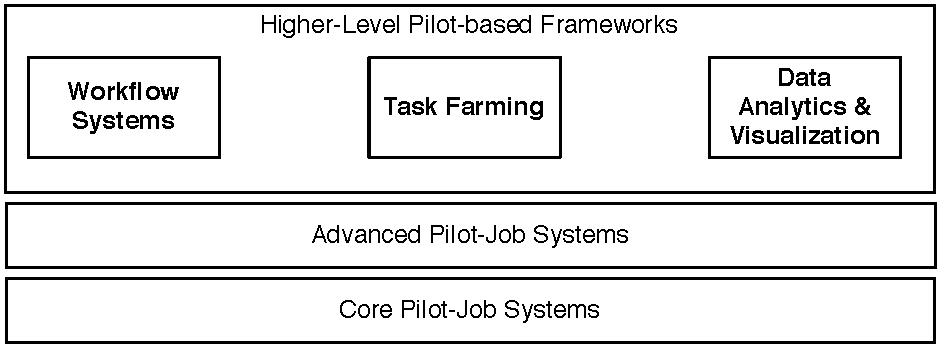
\includegraphics[width=0.45\textwidth]{figures/classification.pdf}
	\caption{Pilot-Job Classification: 	Different PJ systems focus on 
	different parts of the distributed computing stack: (i) PJ systems that 
	solely provide the \pilot capability, (ii) systems that offer resource 
	management capabilities based on \pilots and (iii) applications, tools and 
	services that utilize \pilots for resource management.}
	\label{fig:figures_classification}
\end{figure}


\subsubsection*{Pilot-Job Systems Overview}

PJ to survey (pilots can fall potentially in on or more categories):
\begin{itemize}
	\item Simple Pilot-Job Systems:
	\begin{itemize}
		\item Condor-G/Glide-In
		\item MyCluster (supports both Condor and SGE clusters)
		\item ToPoS 
		\item Co-Pilot
	\end{itemize}
	\item Pilot-based Resource Management Systems
	\begin{itemize}
		\item GlideinWMS
		\item GWPilot??
		\item Dirac?
        \item PanDA  
	\end{itemize}
	\item Higher-Level Application Frameworks (with PJ capabilities):
	\begin{itemize}
		\item Workflow
		\begin{itemize}
			\item Swift/Coaster
			\item Pegasus
		\end{itemize}
		\item Task Farming
		\begin{itemize}
			\item Nimrod/G 
			\item DIANE
			\item Falkon 
		\end{itemize}
		\item Data Analytics \& Visualization
		\begin{itemize}
			\item Bosco
			\item iPython
		\end{itemize}
	\end{itemize}
\end{itemize}

One popular implementation of a \pilotjob is Condor Glide-in~\cite{condor-g}.
Glide-in is a mechanism by which user can add remote grid resources to the
local condor pool and run their jobs on the added resource the same way that
all condor jobs are submitted. The resources added are available only for the
user who added the resource to the pool, thus giving complete control over the
resources for managing jobs without any queue waiting time. Glide-in installs
and executes necessary Condor daemons and configuration on the remote
resource, such that the resource reports to and joins the local Condor pool.
Glide-in is limited in that the daemons must be running on a given resource,
meaning that this process must be approved by resource owners or system
administrators.

Given the interest and uptake of clouds, it is natural that the resource
balancing approaches of \pilotjobs would be employed for clouds too.
\pilotjobs were used at CERN on grid infrastructure to process experiments 
performed with the Large Hadron Collider~\cite{copilot-tr}. 
A desire to utilize a wider variety of computing resources, including enterprise and private clouds, to analyze such experiments drove the creation 
of Co-Pilot~\cite{copilot-tr}, which acts as a layer on top of existing
grid/batch systems to allow job submission to clouds such as Amazon
EC2 or Scientific Clouds. CoPilot uses XMPP messaging to communicate between
the VMs and the grid infrastructure. Co-Pilot is based more on the actual
submission of jobs and is limited in its user-level controllability and 
allowance of application-level programming.

The Coaster system~\cite{coasters} is another \pilotjob implementation
which has been shown to work in both cloud and grid
environments. Using the Coaster service, one executes a Coaster Master
on a head node, and the Coaster workers run on compute nodes to
execute jobs. Coasters offers a zero-install feature in which it
deploys itself and installs itself from the head node and onto the
virtual machines without needing any prior installation on the
machine. In cloud mode, Coasters does require initial installation to
a head node. Coasters uses the CoG kit abstraction library for gram,
ssh, Condor, PBS, SGE middleware connections.
 
Venus-C~\cite{venusc-generic-worker} provides a \pilotjob-like
capability on Microsoft Azure clouds called a Generic Worker. The
Generic Worker creates a layer of abstraction above the inner workings
of the cloud.  The idea behind the Generic Worker is to allow
scientists to do their science without requiring knowledge of backend
HPC systems by offering e-Science as a service. Venus-C has not been
shown to work with grids, because its main objective is to motivate
scientists to use cloud infrastructures.  While the notion of moving
to the cloud for data-driven science is an important one, many
existing cyberinfrastructures still have powerful grid computers that
can also be leveraged to assist with the data-driven computations.

Co-Pilot, Coasters, and the Venus-C Generic Worker vary greatly in
their implementation details, but are all focused on extending
\pilotjob-like capabilities from grids to clouds.

\section{Understanding the Landscape: Developing a Vocabulary}
\mtnote{MT/AZ}

\jhanote{Having surveyed now let us develop the vocabulary.}
\jhanote{I think the main framework + concepts from P* can be used
  here? Any reason not to? What else can be used?}

\begin{itemize}
	\item Distinction between PJ implementation and abstractions;
        \item lack of a unifying model for PJ abstractions;
        \item P* fills the gap;
        \item P* description.
\end{itemize}

\subsection{Different components of the Landscape}

\jhanote{Something akin to Matteo's diagram}

\begin{itemize}
        \item PJ abstractions are not defined in a void;
	\item use cases, scientific practice and distributed applications;
        \item heterogeneous DIs: grid, cloud and hybrids;
	\item jobs and services;
        \item LoAs implied by the PJ abstractions;
	\item diagram.
\end{itemize}

\subsection{Common Terms and Definitions}

\alnote{What to do with the term many-task computing}

\begin{itemize}
	\item application
	\item workflow
        \item pilot
        \item pilot framework
        \item agent, executor
	\item manager
        \item scheduler
	\item job
        \item workload
	\item ensemble
    \item compute unit
	\item platform
\end{itemize}

\section{Pilot-Job Systems Revisited}
\aznote{Ashley's section}
Despite the apparent diversity in existing Pilot-Jobs,
they can be reduced to a set of common functionality and
discussed as such.  This reduction has implications
for the interoperability of existing and future Pilot-Jobs, and
lends insight into application design to enhance job/data(?)
mobility, management, and potential run-time responsiveness via
late-binding/etc.
\subsection{Comparing Pilot-Jobs via a Common Framework \& Vocabulary}
\aznote{Ashley's section}
\jhanote{Having developed the vocabulary let us now talk about the
  different \pilotjobs}
%\mrnote{I don't like calling it understanding pilot jobs. I think by
%now in the paper one should understand}
%\aznote{Here are some suggestions from me: ``Pilot-Jobs in context'',
%``Understanding Pilot-Jobs via the P* Model'', ``Existing
%Pilot-Jobs in light of the P* model'', ``Classifying and 
%Comparing Pilot-Jobs''...  none of these are perfect I think, but I
%think I like no.2 best}
%\aznote{Revisit previous pilot-jobs using the vocabulary from the
%previous section, pointing out the commonalities and overlap.}

%\aznote{Example: Diane's RunMaster covers the role of the Pilot-Manager, and
%the Pilot-Job is handled by Diane's worker agent.  This is similar to the 
%BigJob and Swift-Coaster Pilot-Job implementations.  Condor-G may appear
%different because of X, but in actuality...}

\subsubsection{DIANE}
\aznote{Section copied and pasted from IPDPS paper for now -- plan
to use this general sort of information + reword using our spiffy 
P* vocabulary}
% Coordination and Communication
DIANE~\cite{Moscicki:908910} is a task coordination framework, which
was originally designed for implementing master/worker applications,
but also provides PJ functionality for job-style executions. DIANE
utilizes a single hierarchy of worker agents as well as a PJ manager
referred to as \texttt{RunMaster}.
%Further, there is ongoing work on a multi-master extension.
For the spawning of PJs a separate script, the so-called submitter script, is
required. For the access to the physical resources the GANGA
framework~\cite{Moscicki20092303} can be used.
%GANGA provides a
%unified interface for job submissions to various resource types, e.\,g.\ EGI
%resources or TG resources via a SAGA backend.
Once the worker agents are started they register themselves at the RunMaster.
In contrast to TROY-BigJob, a worker agent generally manages only a single
core and thus, by default is not able to run parallel applications (e.\,g.\
based on MPI). BJ utilizes the BJ-Agent that is able manage a set of local
resources (e.\,g.\ a certain number of nodes and cores) and thus, is capable
of running parallel applications. For communication between the RunMaster and
worker agents point-to-point messaging based on CORBA~\cite{OMG-CORBA303:2004}
is used. CORBA is also used for file staging, which is not fully supported by
BJ, yet.

% Binding 
DIANE is primarily designed with respect to HTC environments (such as
EGI~\cite{egi}), i.\,e.\ one PJ consists of a single worker agent with the
size of 1 core. BJ in contrast is designed for HPC systems such as TG,
where a job usually allocates multiple nodes and cores. To address this issue
a so-called multinode submitter script can be used: the scripts starts a
defined number of worker agents on a certain resource. However, WUs will be
constrained to the specific number of cores managed by a worker agent. A
flexible allocation of resource chunks as with BJ is not possible. By
default a WU is mapped to a SU; application can however implement smarter
allocation schemes, e.\,g.\ the clustering of multiple WUs into a SU.

%Scheduling
DIANE includes a simple capability matcher and FIFO-based task scheduler.
Plugins for other workloads, e.\,g.\ DAGs or for data-intensive
application, exist or are under development. The framework is extensible:
applications can implement a custom application-level scheduler.


%Other impl. related issues: FT and security
DIANE is, just like BJ, a single-user PJ, i.\,e.\ each PJ is executed with the
privileges of the respective user. Also, only WUs of this respective user can be
executed by DIANE. DIANE supports various middleware security mechanisms
(e.\,g.\ GSI, X509 authentication). For this purpose it relies on GANGA. The
implementation of GSI on TCP-level is possible, but currently not yet
implemented. Further, DIANE supports fault tolerance: basic error detection and
propagation mechanisms are in place. Further, an automatic re-execution of WUs
is possible.

%\upp
\subsubsection{Condor-G}
\aznote{Section copied and pasted from IPDPS paper for now -- plan
to use this general sort of information + reword using our spiffy 
P* vocabulary}
Condor-G pioneered the Pilot-Job concept~\cite{condor-g}. The pilot is
actually a complete Condor pool that is started using the Globus
service of a resource. This mechanism is referred to as Condor
Glide-In. Subsequently, jobs can be submitted to this Glide-In pool
using the standard Condor tools and APIs. Condor utilizes a
master/worker coordination model. The PJ manager is referred to as the
Condor Central Manager. The functionality of the Central Manager is
provided by several daemons: the condor\_master that is generally
responsible for managing all daemons on a machine, the
condor\_collector which collects resource information, the
condor\_negotiator that does the matchmaking and the condor\_schedd
that is responsible for managing the binding and scheduling
process. Condor generally does not differentiate between workload,
i.\,e.\ WU, and schedulable entity, i.\,e.\ SU. Both entities are
referred to as job. However, it supports late binding, i.\,e.\
resources a job is submitted to must generally not be available at
submission time. The scheduler matches the capabilities required by a
WU to the available resources. This process is referred to as
matchmaking. Further, a priority-based scheduler is used. For
communication between the identified elements Condor utilizes
point-to-point messaging using a binary protocol on top of TCP.

Different fault tolerance mechanisms, such as automatic retries, are
supported.  Further, Condor supports different security mechanisms:
for authentication it integrates both with local account management
systems (such as Kerberos) as well as grid authentication systems such
as GIS. Communication traffic can be encrypted.

\subsubsection{Swift}
\aznote{Material on Swift goes here}

\subsubsection{GWPilot}
%\begin{lstlisting}[breaklines]
\url{https://indico.egi.eu/indico/materialDisplay.py?contribId=18&sessionId=46&materialId=slides&confId=1019}
\\
\url{http://ieeexplore.ieee.org/xpls/abs_all.jsp?arnumber=6266981}
%\end{lstlisting}

\subsubsection{Bosco}
\url{http://iopscience.iop.org/1742-6596/396/3/032116/pdf/1742-6596_396_3_032116.pdf}

% \upp
% \subsection{SWIFT-Coaster\upp\upp}
% 
% SWIFT~\cite{Wilde2011} is a scripting language designed for expressing abstract
% rest of this cut, but making a note of this in case we want
% to bring swift into the discussion later that i can find more info in 2011 paper
%\aznote{Much of what I was thinking of doing is similar to the 2011 IPDPS paper
%in the 2012-PStar directory.  Is this along the right lines?}

%\aznote{A bit confused about how to tie this into conclusion and discussion:
%``The need for a common minimum model'' in particular.  I am guessing that
%I should help to ``set up'' that section by providing plenty of material showing
%that the pilot job systems are very similar at their core.  How far should I
%go with this, however, to avoid hitting the ``conclusion'' material in this section?
%}

\section{Conclusion and Discussion}

\subsection{The need for a common minimum model}

%Whereas we will discuss in greater detail some of the concepts upon
%which this paper is built, for completeness we briefly outline them
%here.

Once a common and uniform conceptual model was available, the notion
of \pilotdata was conceived using the power of symmetry, i.e., the
notion of \pilotdata was as fundamental to dynamic data placement and
scheduling as \pilotjobs was to computational tasks. As a measure of
validity, the \pstar model was amenable and easily extensible to
\pilotdata.  The consistent and symmetrical treatment of data and
compute in the model led to the generalization of the model as the
{\it P* Model of Pilot Abstractions}.


\subsection{Lessons for Workflow System}

The current state of workflow (WF) systems~\cite{nsf-workflow,1196459}
provides a motivating example for the P* Model and the Pilot-API: even
though many WF systems exist (with significant duplicated effort),
they provide limited means for extensibility and interoperability.  We
are not naive enough to suggest a single reason, but assert that one
important contributing fact is the lack of the right interface
abstractions upon which to construct workflow systems; had those been
available, many/most WF engines would have likely utilized them (or
parts thereof), instead of proprietary solutions.

% That would not immediately allow WF implementations to interoperate,
% but would make semantic mapping between them significantly simpler,
% thus supporting the very notion of interoperation.

Significant effort has been invested towards WF interoperability at
different levels -- if nothing else, providing post-facto
justification of its importance. The impact of missing interface
abstractions on the WF world can be seen through the consequences of
their absence: WF interoperability remains difficult if not
infeasible. The Pilot-API in conjunction with the P* Model aims to
prevent similar situation for \pilotjobs.

%\footnote{To be fair: we are not sure if a generic model and/or a
%  generic WF API are achievable {\it on a useful level} -- we think,
%  nevertherless, that our discussion is valid.}



\section{Related Work}

\mrnote{We have a survey of related \pilotjobs systems, a 
'history' of \pilotjobs, and a related work section? Not sure
if we should condense in some way. PS Why is this after conclusion?}

\subsection{Scientific Data Management}



\section*{Acknowledgements}
This work is funded by NSF CHE-1125332 (Cyber-enabled Discovery and
Innovation), NSF-ExTENCI (OCI-1007115) and ``Collaborative Research:
Standards-Based Cyberinfrastructure for Hydrometeorologic Modeling:
US-European Research Partnership'' (OCI-1235085) and Department of
Energy Award (ASCR) DE-FG02-12ER26115.  This work has also been made
possible thanks to computer resources provided by TeraGrid TRAC award
TG-MCB090174 and BiG Grid.  This document was developed with support
from the US NSF under Grant No. 0910812 to Indiana University for
``FutureGrid: An Experimental, High-Performance Grid Test-bed''.

% \bibliographystyle{IEEEtran}
\bibliographystyle{abbrv}
\bibliography{pilotjob,literatur,saga,saga-related}


\end{document}

